\documentclass[11pt]{article}

\usepackage[margin=1in]{geometry}
\usepackage{amsmath}
\usepackage{booktabs}
\usepackage{graphicx}
\usepackage{microtype}
\usepackage{hyperref}
\usepackage{xcolor}

\hypersetup{
  colorlinks=true,
  linkcolor=blue!50!black,
  citecolor=blue!50!black,
  urlcolor=blue!60!black
}
\graphicspath{{figures/}}

\title{Assignment 1: Membership Inference Attacks}
% Add team member names before submission if required.
\author{}
\date{Fall 2026}

\begin{document}
\maketitle

\begin{abstract}
This report evaluates membership inference against a neural classifier trained on a
privacy-sensitive synthetic health-care dataset. We generate 9,000 labelled hospital
encounters with a class-conditional mixed-type diffusion model, train a target classifier
on 3,000 records, and reserve 6,000 records as nonmembers. We then compare negative-loss
and true-class-logit attacks with offline LiRA using 128 shadow models. Offline LiRA
achieves an ROC AUC of 0.5976 and a true-positive rate of 4.2\% at 1\% false-positive
rate, outperforming both baselines in the low-false-positive regime. Ablations show
diminishing returns beyond 64 shadows and substantially greater leakage as the target
model overfits. We conclude with an analysis of the additional conceptual, statistical,
and societal challenges posed by membership inference against frontier generative models.
\end{abstract}

\section{Threat Model and Experimental Scope}

We use the assignment's grey-box threat model. The attacker observes target-model outputs
such as logits or losses and knows the architecture and training procedure, but does not
know the target weights or membership labels. The attacker has a separate pool drawn from
the same synthetic distribution for training shadow models.

The membership question in Tasks A and B is whether a synthetic encounter was used to
train the target classifier. It is not a claim about whether a real patient was used to
train the synthetic-data generator. Synthetic outcomes are generated labels rather than
verified clinical outcomes, and the procedure provides no formal privacy guarantee.

\section{Task A: Dataset and Target Model}

\subsection{Data source and privacy-sensitive use case}

The source is the UCI Diabetes 130-US Hospitals dataset, a CC BY 4.0 collection of
inpatient encounters with demographic, diagnostic, medication, and 30-day readmission
information \cite{uci-diabetes}. The use case is prediction of readmission within 30 days
from information available at discharge. Hospice and expired discharge dispositions are
removed because a positive 30-day readmission is not meaningful for these encounters.
Patient identifiers are used only to create disjoint real-data partitions and never enter
the generator or classifier.

The binary target is one for readmission within 30 days (\texttt{<30}) and zero for later
or no readmission. Raw \texttt{?} values are treated as missing, literal \texttt{None}
laboratory results are represented as \texttt{not\_measured}, and diagnosis codes are
grouped into broad clinical categories. Administrative codes are treated as categorical
rather than ordinal. Missing categorical values receive an explicit level, and core
category levels occurring fewer than 25 times are grouped using generator-training data
only.

Patients are divided into approximately 70\%/15\%/15\% generator-training, validation, and final
utility-test groups with no patient overlap. From these partitions, 25,000, 10,000, and
10,000 encounters are used, respectively. The generator retains eight encounter-count
variables, a compact group of demographic and clinical categorical variables, and every
nonconstant diabetes-medication field.

\subsection{Synthetic-data generator}

We train a compact, class-conditional TabDDPM inspired by Kotelnikov et al.
\cite{tabddpm}. Numerical counts are mapped through a Gaussian quantile transform and
diffused with a Gaussian forward process. Each categorical column retains its own
vocabulary and multinomial diffusion process. The readmission outcome is excluded from
the generated vector and supplied to the denoising network as a class condition.

The quantile transform and categorical vocabularies are learned from the generator-training
partition only. After sampling, numerical values are inverse-transformed, rounded to valid
integer counts, and clipped to the observed training bounds. The fields \texttt{change}
and \texttt{diabetesMed} are then reconstructed from the generated medication states.

The denoiser is a four-block residual multilayer perceptron of width 512. It receives the
noisy mixed record, a sinusoidal embedding of the diffusion timestep, and a learned label
embedding. It is trained for 20,000 steps with 200 diffusion steps, batch size 1,024,
AdamW learning rate $2\times10^{-4}$, and exponential-moving-average decay 0.999.
Balanced training batches ensure that the minority class is learned; sampling then restores
the empirical class prevalence. Following the dependency-aware reconstruction idea in
Umesh et al. \cite{hfgf}, reconstructing the two derived medication fields avoids
generating logically inconsistent combinations.

The generator produces 9,000 unique records with a positive-label prevalence of 0.1122.
The class counts match the generator-training prevalence. Full duplicates and exact
matches to generator seed rows are discarded and resampled. This is a conservative data
hygiene check, not a formal privacy test.

\subsection{Synthetic-data quality}

Quality is assessed through selected marginals, grouped readmission relationships,
logical consistency, duplicate and seed-match audits, and train-on-synthetic/test-on-real
(TSTR) utility. Table~\ref{tab:marginals} shows that total-variation distance is small for
the reviewed marginals. The largest observed value is 0.0249 for age. The audit finds no
full duplicates, exact generator-seed matches, medication inconsistencies, or excluded
discharge dispositions.

\begin{table}[htbp]
\centering
\caption{Selected synthetic-versus-real marginal differences.}
\label{tab:marginals}
\begin{tabular}{lrr}
\toprule
Feature & Total variation & Largest category gap \\
\midrule
Gender & 0.0005 & 0.0005 \\
Age & 0.0249 & 0.0128 \\
Race & 0.0091 & 0.0057 \\
Insulin & 0.0054 & 0.0054 \\
A1C result & 0.0060 & 0.0060 \\
Target & 0.0088 & 0.0088 \\
\bottomrule
\end{tabular}
\end{table}

\IfFileExists{figures/synthetic_quality.png}{
\begin{figure}[htbp]
  \centering
  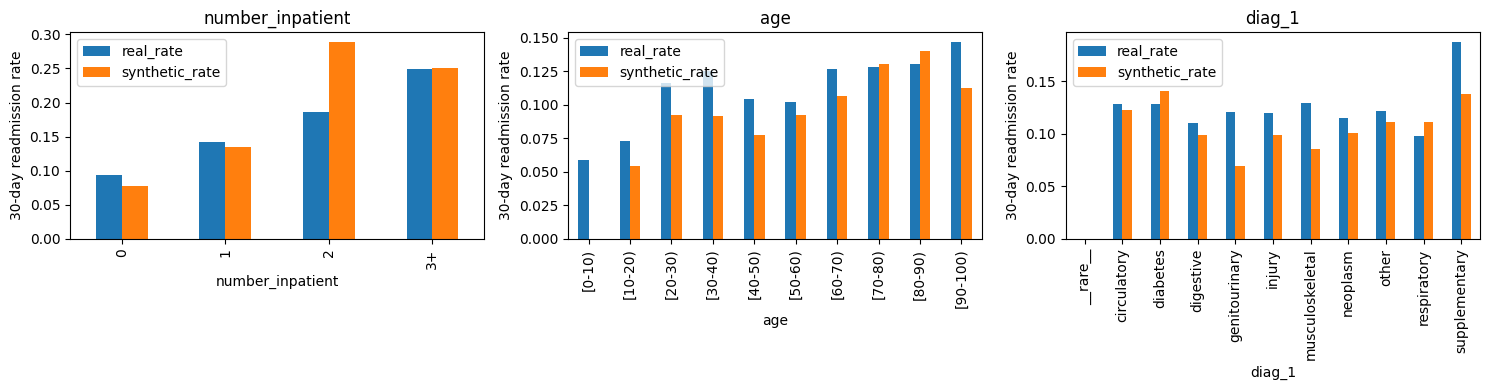
\includegraphics[width=0.95\linewidth]{synthetic_quality.png}
  \caption{Selected numerical distributions and readmission relationships in the real and synthetic data.}
  \label{fig:synthetic-quality}
\end{figure}
}{}

Matched logistic-regression models are trained on 3,000 real or synthetic encounters and
evaluated on an untouched 10,000-record real-patient test partition. As shown in
Table~\ref{tab:utility}, TSTR utility remains above chance but is weaker than direct
real-data training. These results support use of the frozen dataset for the assignment,
but not a claim that the synthetic data are clinically equivalent to the source data.

\begin{table}[htbp]
\centering
\caption{Train-on-real/test-on-real (TRTR) and train-on-synthetic/test-on-real (TSTR) utility.}
\label{tab:utility}
\begin{tabular}{lrrrrr}
\toprule
Experiment & Accuracy & Balanced accuracy & Average precision & AUROC & Cross-entropy \\
\midrule
TRTR & 0.8840 & 0.5159 & 0.1956 & 0.6139 & 0.3527 \\
TSTR & 0.8841 & 0.5129 & 0.1715 & 0.5888 & 0.3699 \\
\bottomrule
\end{tabular}
\end{table}

\subsection{Membership split and target classifier}

The frozen synthetic dataset is randomly divided using label stratification into 3,000 target
members and 6,000 nonmembers. Stable record identifiers are metadata and are not model
inputs. The target is a two-hidden-layer multilayer perceptron with widths 128 and 64,
trained for 50 epochs with batch size 128, Adam learning rate $10^{-3}$, weight decay
$10^{-5}$, and unweighted cross-entropy. Numerical inputs are median-imputed and
standardized using statistics fitted only on the model's training records. Categorical
inputs are one-hot encoded with the generator-training schema, with unseen levels ignored.
The numerical preprocessing is refitted independently for the target and every shadow
model, preventing evaluation records from influencing the learned transformation.

The target reaches 1.0000 training AUROC and 0.7031 nonmember-test AUROC. Its training
accuracy is 1.0000 compared with 0.8603 on nonmembers, producing a pronounced fitting gap
that Task B examines directly.

\section{Task B: Baseline Attacks and Offline LiRA}

\subsection{Attack signals and evaluation}

For a labelled record $(x,y)$, the LOSS attack uses negative cross-entropy,
\begin{equation}
  s_{\mathrm{loss}}(x,y)=-\ell(f(x),y),
\end{equation}
so that larger scores indicate stronger membership evidence. The second baseline uses the
pre-softmax logit for the true class. LiRA instead uses the logit margin
\begin{equation}
  \phi(x,y)=z_y-\log\sum_{k\ne y}\exp(z_k).
\end{equation}
For each candidate, only shadow models that did not train on it define the Gaussian OUT
distribution. The offline LiRA score is the Gaussian CDF of the target statistic under
that fitted OUT distribution. We evaluate both a per-record variance estimate and a
fixed-variance alternative.

Balanced accuracy is reported at the best empirical ROC threshold and is therefore
descriptive. ROC AUC and true-positive rate (TPR) at 0.1\%, 1\%, 5\%, and 10\%
false-positive rate (FPR) provide threshold-independent and operationally low-FPR views.
All scores are oriented so larger values indicate stronger membership evidence.

\subsection{Shadow-model design}

We train 128 shadow models using the target architecture, optimizer, batch size, and
unweighted loss. Each shadow trains on a different 3,000-record half of the 6,000
nonmember pool; target members never enter shadow training. Complementary random pairs
ensure that every even prefix of the shadow ensemble is balanced. Every target member has
128 OUT observations, while each nonmember has 64. This count difference is not used as
an attack feature.

Numerical preprocessing is fitted independently on each shadow's training records. One
50-epoch trajectory saves checkpoints at 1, 15, and 50 epochs for the fitting ablation.
This makes the ablation efficient and fixes the data, initialization, architecture,
optimizer, and preprocessing within each trajectory.

\subsection{Primary attack results}

Table~\ref{tab:attacks} reports the primary results. Offline LiRA achieved the highest AUC, 0.5976, compared with 0.5665 for LOSS and 0.5671 for the true-class logit. The difference was larger at low FPR. At 1\% FPR, LiRA identified 4.2\% of members, while LOSS identified none and the logit attack identified 1.27\%.

LiRA's best-threshold balanced accuracy is lower because the ROC curves cross: balanced
accuracy evaluates one empirically selected threshold, whereas AUC measures ranking over
all thresholds. For membership inference, AUC and low-FPR performance are more informative
because false accusations must be rare. The improvement is nevertheless modest; an AUC of
0.5976 is above chance but is not strong evidence of membership for an individual record.

\begin{table}[htbp]
\centering
\small
\caption{Membership-inference performance on 3,000 members and 6,000 nonmembers.}
\label{tab:attacks}
\begin{tabular}{lrrrrrr}
\toprule
Attack & Balanced acc. & AUC & TPR@0.1\% & TPR@1\% & TPR@5\% & TPR@10\% \\
\midrule
LOSS & 0.6164 & 0.5665 & 0.0000 & 0.0000 & 0.0523 & 0.1033 \\
True-class logit & 0.6169 & 0.5671 & 0.0010 & 0.0127 & 0.0523 & 0.1030 \\
Offline LiRA & 0.5615 & 0.5976 & 0.0080 & 0.0420 & 0.1250 & 0.1987 \\
LiRA, fixed variance & 0.5625 & 0.5932 & 0.0093 & 0.0310 & 0.1117 & 0.1943 \\
\bottomrule
\end{tabular}
\end{table}

\IfFileExists{figures/attack_roc.png}{
\begin{figure}[htbp]
  \centering
  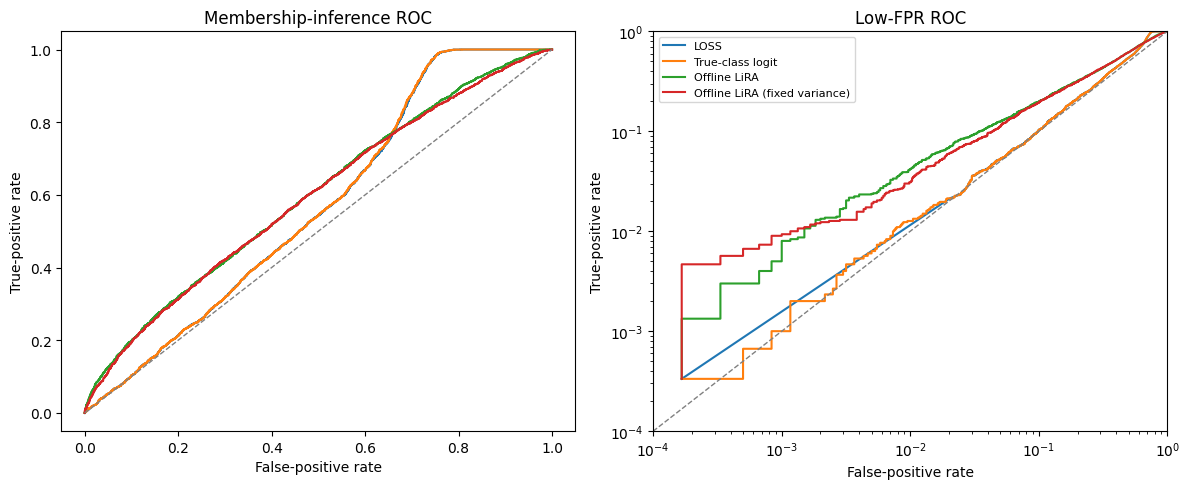
\includegraphics[width=0.9\linewidth]{attack_roc.png}
  \caption{Membership-inference ROC curves, with a log-scale low-FPR view.}
  \label{fig:attack-roc}
\end{figure}
}{}

\subsection{Shadow-count ablation}

The shadow-count ablation reuses nested prefixes of 8, 16, 32, 64, and 128 cached
models. Table~\ref{tab:shadow-ablation} shows that per-record-variance AUC increases from
0.5890 with 8 shadows to 0.5976 with 128, with diminishing improvement beyond 64.
Per-record variance is noisy with very small ensembles because each record has only four
OUT samples at $N=8$; fixed variance is correspondingly more stable in that regime.

\begin{table}[htbp]
\centering
\caption{Offline LiRA shadow-count ablation.}
\label{tab:shadow-ablation}
\begin{tabular}{rrrrrr}
\toprule
Shadows & Min. OUT & AUC & TPR@0.1\% & TPR@1\% & TPR@10\% \\
\midrule
8   & 4  & 0.5890 & 0.0000 & 0.0057 & 0.1377 \\
16  & 8  & 0.5935 & 0.0003 & 0.0197 & 0.1760 \\
32  & 16 & 0.5958 & 0.0073 & 0.0303 & 0.1963 \\
64  & 32 & 0.5960 & 0.0027 & 0.0367 & 0.1950 \\
128 & 64 & 0.5976 & 0.0080 & 0.0420 & 0.1987 \\
\bottomrule
\end{tabular}
\end{table}

\IfFileExists{figures/shadow_count_ablation.png}{
\begin{figure}[htbp]
  \centering
  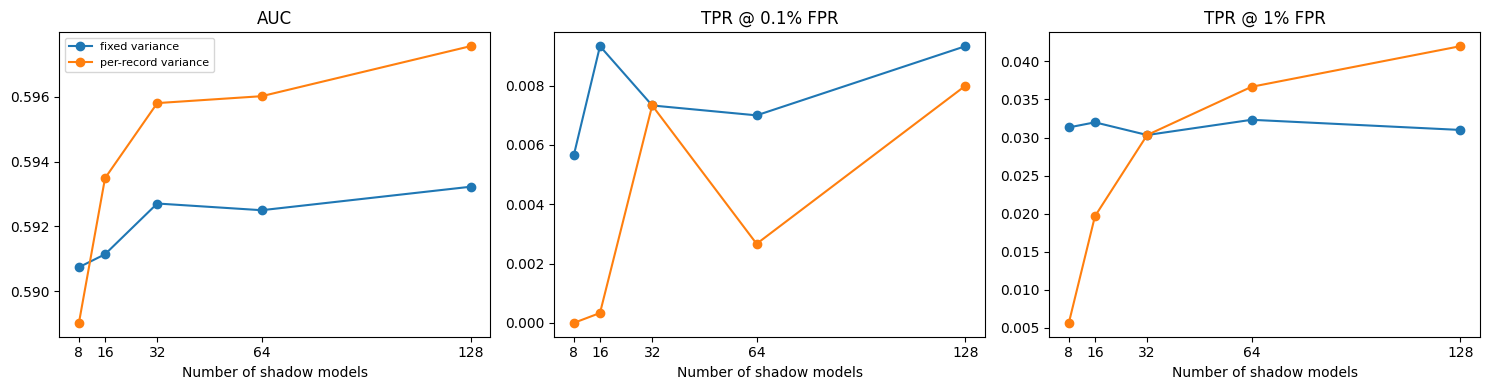
\includegraphics[width=0.95\linewidth]{shadow_count_ablation.png}
  \caption{Effect of shadow-model count on offline LiRA.}
  \label{fig:shadow-count}
\end{figure}
}{}

\subsection{Underfitting and overfitting ablation}

The target and shadows are evaluated at matched 1-, 15-, and 50-epoch checkpoints.
Table~\ref{tab:fitting-ablation} shows that leakage grows with fitting. LiRA is essentially
random at one epoch, reaches 0.5659 AUC at 15 epochs, and reaches 0.5976 at 50 epochs.
Over the same checkpoints, the target accuracy gap grows from approximately zero to
0.1397 and the cross-entropy gap grows to 0.9037. Overfitting therefore creates a much
stronger record-specific signal, although aggregate target test AUROC changes little
between 15 and 50 epochs.

\begin{table}[htbp]
\centering
\caption{Fitting ablation with matched target and shadow checkpoints.}
\label{tab:fitting-ablation}
\begin{tabular}{lrrrrrr}
\toprule
Regime & Epochs & Accuracy gap & CE gap & LOSS AUC & Logit AUC & LiRA AUC \\
\midrule
Underfit & 1  & -0.0002 & -0.0002 & 0.4969 & 0.4957 & 0.4984 \\
Intermediate & 15 & 0.0423 & 0.1943 & 0.5271 & 0.5273 & 0.5659 \\
Overfit & 50 & 0.1397 & 0.9037 & 0.5665 & 0.5671 & 0.5976 \\
\bottomrule
\end{tabular}
\end{table}

\IfFileExists{figures/fitting_ablation.png}{
\begin{figure}[htbp]
  \centering
  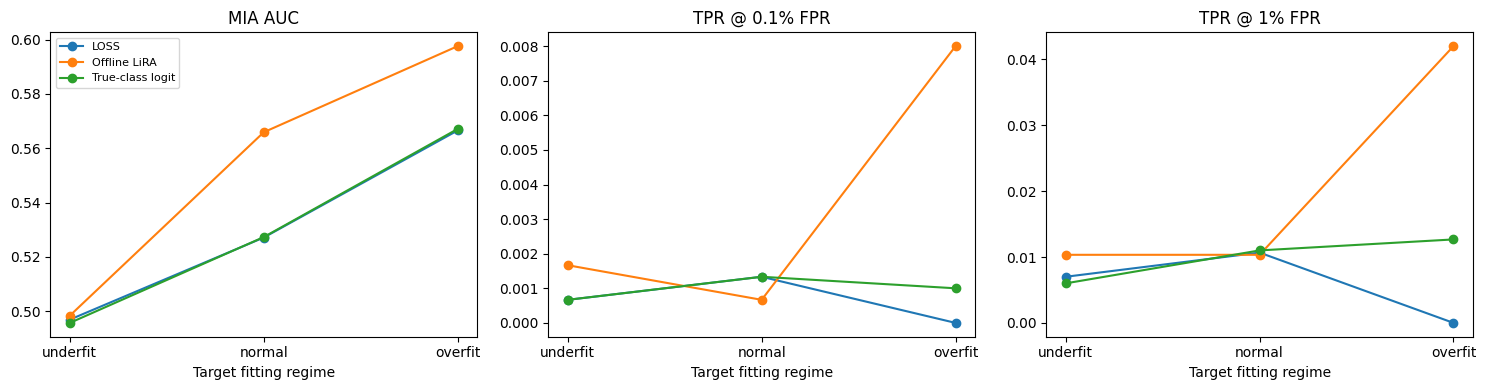
\includegraphics[width=0.95\linewidth]{fitting_ablation.png}
  \caption{Attack performance across matched target/shadow fitting regimes.}
  \label{fig:fitting}
\end{figure}
}{}

This is a single-query offline attack adapted to tabular classification. We do not use
image-style augmentations because no defensible label-preserving tabular perturbation was
defined. The implementation follows the central offline-LiRA design of Carlini et al.
\cite{lira} and uses cached scores, per-example Gaussian fitting, a fixed-variance
comparison, and log-scale ROC reporting.

\section{Task C: Membership Inference for Generative AI}

Membership inference asks whether a specified unit appeared in training. It is distinct
from extraction, which reconstructs training content, and attribution, which asks whether
a training unit caused a particular output. Evidence for one does not establish the others.

\subsection{Why generative-model membership inference is harder}

For classifiers, we can often use loss or confidence as a membership signal. Generative models do not provide such a clean signal. Their outputs also change with prompts, decoding settings, and random seeds, so it is harder to separate membership effects from ordinary generation variability.

The training scale also dilutes individual influence. Duplicates and semantically similar
records let a model learn the same pattern without depending on one example, while matched
reference models are expensive and difficult to construct. In a large-scale study, strong
language-model attacks remained below 0.7 AUC and many per-example decisions were unstable
\cite{hayes2025}. The membership unit itself may be ambiguous: a span, document, image,
person, or creator defines a different claim. Dai and Gifford further show that
leave-one-out attribution for diffusion outputs weakens as training sets grow
\cite{dai2026}. Thus, output similarity alone is not reliable evidence of membership or
causal influence.

\subsection{Effect of modality}

\paragraph{Text.} Token probabilities permit sequence-level or low-probability-span
scores, but paraphrases, overlapping documents, tokenization, and uncertain document
boundaries complicate membership.

\paragraph{Images.} Diffusion generation is stochastic and has no unique classifier-loss
analogue. Pixel distance may reject equivalent images, while embedding distance may miss
copied details; prompts and random seeds must therefore be controlled.

\paragraph{Audio and video.} These inherit image-similarity problems and add temporal
alignment and segmentation choices.

\paragraph{Structured records.} Fixed fields and clear row boundaries make membership
closer to Task B, although an attacker must still distinguish an exact row from a person
represented by several rows or a population property.

The main difference between modalities is what counts as ``the same example.'' For text,
paraphrases may preserve meaning; for images, small pixel changes may still represent the
same image; for audio and video, timing and segmentation add another layer.

\subsection{Interested parties}

Data subjects and creators could investigate unauthorized use of their records or work.
Auditors, regulators, researchers, and developers could test dataset disclosures,
memorization, removal, or unlearning. Journalists and litigants might use validated results
as supporting evidence, although MIA alone does not prove infringement or causation.
Malicious actors could instead reveal participation in a sensitive dataset or select
targets for extraction and re-identification. MIA is therefore both an accountability tool
and a privacy attack.

\subsection{How an attacker could improve success}

An attacker can improve success by targeting rare or duplicated examples, conditioning on
known prefixes or metadata, and calibrating each candidate with matched reference models.
An attacker can query the same example in several controlled ways and combine the results. However, those queries are correlated, so they cannot be treated as independent evidence. Group-level tests can combine weak signals across one person
or creator, but they change the claim and its base rate. Legitimate access to
log-probabilities, gradients, checkpoints, or denoising trajectories can also help.

Calibrated filtering has enabled extraction of verbatim text from GPT-2
\cite{carlini2021} and training images from diffusion models \cite{carlini2023}. These
results show memorization risk, but extraction success does not imply reliable membership
decisions for ordinary records.

\subsection{Societal impacts}

A reliable MIA could be useful for accountability. For example, creators could test whether their work was included in an undisclosed training dataset, or auditors could check whether data claimed to be deleted or unlearned still influences a model. This is a real concern: in an FTC discussion on generative AI, creators reported that they often cannot tell whether their work was used for training because model developers do not disclose their training data \cite{ftc2023}.

The same capability could expose participation in a sensitive medical or legal dataset
without reconstructing the underlying record. Even a small FPR could produce many false
accusations at population scale. Results should therefore report low-FPR performance,
uncertainty, base rates, stability, and corroborating evidence.

For copyright disputes, a positive result may support a claim that a work was accessed,
but it does not prove that a particular output copied or was caused by that work. A
negative result likewise does not prove absence because current attacks have limited
power. MIA should therefore be treated as a probabilistic audit tool alongside provenance,
documentation, extraction testing, and legal fact-finding.

\section{Conclusion}

Offline LiRA provides a measurable advantage over loss and logit baselines on the frozen
synthetic health-care classifier, especially at low false-positive rates. More shadow
models improve the estimate, but gains diminish after roughly 64 models. The fitting
ablation supplies the clearest result: record-level leakage increases substantially as the
target memorizes its training set. However, the final AUC of 0.5976 remains a weak attack
in absolute terms and should not be treated as definitive evidence about one record.

Membership inference against frontier generative models is neither generally impossible
nor reliably solved. It is strongest for atypical or repeated examples, matched reference
distributions, informative model outputs, and controlled repeated queries. Its limits are
equally important: redundant corpora dilute individual influence, reference modeling is
expensive, modalities lack a universal score, and per-record decisions can be unstable.
Responsible use requires a precise membership unit, realistic nonmember controls, low-FPR
evaluation, uncertainty reporting, and clear separation of membership, extraction, and
causal attribution.

\appendix
\section{Reproducibility}

The accompanying notebook \texttt{MIA\_Task\_A\_Colab.ipynb} contains the complete
executable Tasks A and B pipeline and saved outputs. It is intended for a Google Colab T4
GPU and mounts Google Drive. Production artifacts are stored under
\texttt{MyDrive/mia\_task\_a/tabddpm\_v1}. The submitted settings are fixed at 9,000
synthetic records, a 50-epoch target model, 128 shadows, and random seed 684. Generator,
target, and shadow
artifacts are cached so interrupted sessions can resume without retraining completed
models. The accompanying \texttt{README.md} gives concise execution instructions.

\begin{thebibliography}{99}

\bibitem{uci-diabetes}
B. Clore, K. Cios, J. DeShazo, and B. Strack.
\newblock Diabetes 130-US Hospitals for Years 1999--2008.
\newblock UCI Machine Learning Repository, 2014.
\newblock \url{https://doi.org/10.24432/C5230J}.

\bibitem{tabddpm}
A. Kotelnikov, D. Baranchuk, I. Rubachev, and A. Babenko.
\newblock TabDDPM: Modelling tabular data with diffusion models.
\newblock In \emph{Proceedings of ICML}, 2023.
\newblock \url{https://proceedings.mlr.press/v202/kotelnikov23a.html}.

\bibitem{hfgf}
S. Umesh et al.
\newblock Dependency-aware synthetic tabular data generation.
\newblock arXiv:2507.19211, 2025.
\newblock \url{https://arxiv.org/abs/2507.19211}.

\bibitem{lira}
N. Carlini, S. Chien, M. Nasr, S. Song, A. Terzis, and F. Tram\`er.
\newblock Membership inference attacks from first principles.
\newblock In \emph{IEEE Symposium on Security and Privacy}, 2022.
\newblock \url{https://arxiv.org/abs/2112.03570}.

\bibitem{hayes2025}
J. Hayes et al.
\newblock Exploring the limits of strong membership inference attacks on large language models.
\newblock In \emph{NeurIPS}, 2025.
\newblock \url{https://papers.nips.cc/paper_files/paper/2025/hash/7f0f3a1d358f8a902b1c4b15a6848d71-Abstract-Conference.html}.

\bibitem{dai2026}
X. Dai and D. Gifford.
\newblock Outputs of generative diffusion models are often unattributable.
\newblock \emph{Nature Communications}, 17, 2026.
\newblock \url{https://www.nature.com/articles/s41467-026-75667-5}.

\bibitem{carlini2021}
N. Carlini et al.
\newblock Extracting training data from large language models.
\newblock In \emph{USENIX Security}, 2021.
\newblock \url{https://www.usenix.org/conference/usenixsecurity21/presentation/carlini-extracting}.

\bibitem{carlini2023}
N. Carlini et al.
\newblock Extracting training data from diffusion models.
\newblock In \emph{USENIX Security}, 2023.
\newblock \url{https://www.usenix.org/conference/usenixsecurity23/presentation/carlini}.

\bibitem{ftc2023}
U.S. Federal Trade Commission.
\newblock FTC staff report details key takeaways from AI and creative fields panel discussion.
\newblock 2023.
\newblock \url{https://www.ftc.gov/news-events/news/press-releases/2023/12/ftc-staff-report-details-key-takeaways-ai-creative-fields-panel-discussion}.

\end{thebibliography}

\end{document}
